\section{Trends in Corn Yield in North America}

Average yields in both Canada and the U.S have been increasing over the entire study period \citep{CANy, NASSy}. Figures 2.1 and 2.2 show the average  corn yields, in both Iowa and Ontario, for the years considered in this study.

\begin{figure}[!hb]
  \centering
  \begin{minipage}[b]{0.45\textwidth}
    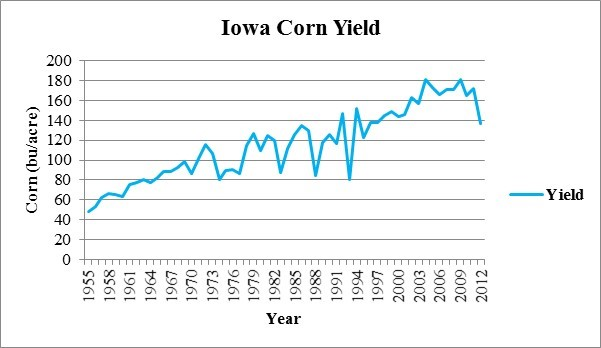
\includegraphics[width=\textwidth]{CornYieldIowa.jpg}
    \caption{Corn Yield (bu per acre) Iowa: 1955-2012 (NASS)}
  \end{minipage}
  \hfill
  \begin{minipage}[b]{0.45\textwidth}
    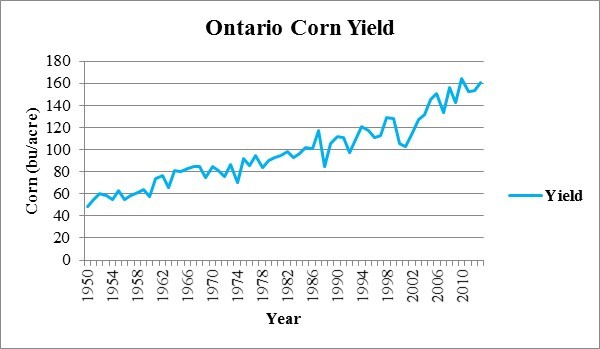
\includegraphics[width=\textwidth]{CornYieldOntario.jpg}
    \caption{Corn Yield (bu per acre) Ontario: 1950-2013 \citep{CANy}}
  \end{minipage}
\end{figure}

These figures show that average yield, in both Ontario and Iowa, has risen substantially over this period. The increase in yield has largely been the result of improved hybrids, and other agricultural technologies \citep{edgerton2009increasing}. In particular, the number of plants per acre has increased at a rate of approximately 400 plants per acre per year over the past 50 years in the central US cornbelt \citep{duvick2005contribution}. Each plant theoretically requires input levels to be within particular ranges and combinations in order to attain a high level of production. Thus, as the number of plants per acre increases, there is likely to be a change in the total level of inputs per acre required to attain relatively high yields. Changes can be made to  agricultural management practices in order to accommodate the needs of increased plants per acre, for example, the amount of fertilizer can be increased, or techniques to improve the water holding capacity can be undertaken. However, some of the inputs affecting corn yield are out of producer control, such as precipitation. Given that poor weather conditions can decimate yields while ideal conditions cannot increase yields beyond their biological potential, corn yield distributions are generally negatively skewed \citep{tolhurst2014technological}. According to \cite{tolhurst2014technological}, yield outcomes can be separated into `regular' and `poor' years in order to reflect this characteristic of yield distributions. The 2011 census of agriculture reports that less than 1\% of all farm acres in Ontario are irrigated \citep{CANirrigation, CANcensus}. In general, almost all corn in North America is grown without irrigation, and therefore water input levels depend almost solely on weather patterns. If a higher level of precipitation per acre is needed to attain high yields, this would increase the likelihood that precipitation will be a limiting factor in any given year.  This could result in an increase in the probability of a `poor' yield year, as precipitation would be a limiting factor more often. At the same time, precipitation levels which are too high can also be damaging. When too much precipitation occurs in a short period of time it can damage crops through flooding as well as by increasing the soil moisture which can heighten the risk of plant disease and infestation, delaying both planting and harvesting \cite{rosenzweig2002increased}. It would be expected that an increase in plants per acre would raise the maximum beneficial level of precipitation,  due to the presumably elevated demand for water. However, the heightened density of plants per acre could also result in higher levels of competition for soil nutrients which could be depleted by heavy rainfall. Therefore, the resulting effects of the interplay of changing agricultural technology, farm management practices, and weather is complex.

\section{Crop Insurance}

Agricultural producers face income uncertainty which can be decreased through participation in programs such as crop insurance. Given that this research is based on yield levels, the crop insurance programs  discussed are those which guarantee yield as opposed to  other measures of producer livelihood such as profit margins or whole farm income. Crop insurance for corn is government subsidized in both Iowa and Ontario in order to help producers access a low cost income risk mitigation tool. As discussed in the introduction, subsidization transfers  a portion of production risk to the public, and is done to increase participation in crop insurance programs. High risk production choices are therefore relatively more attractive to producers than they would be without subsidization, which suggests that production decisions could be distorted by these programs. In \cite{goodwin2013harm}, corn acreage at the county level was found to increase with mean subsidy rate in the US, supporting this claim \citep{goodwin2013harm}. \cite{kerRMP2016} demonstrated that the change in corn yield distributions in Ontario have shifted the upper end of the yield distribution up more quickly than the lower end \citep{kerRMP2016}. This observation is consistent with producers using crop insurance as a substitute for other risk reducing practices. The benefit to producers from subsidized crop insurance is significant, \cite{goodwin2013harm} estimate that in the US ``each dollar of premium paid by farmers tends to yield approximately \$1.90 in indemnity payments". As a result, producers may engage in rent seeking behaviour in order to increase subsidies, or at least prevent their decrease \citep{coble2013we, kerRMP2016}. 

The Production Insurance (PI) program in Ontario and the yield guarantee (YG) program in Iowa provide insurance on the total level of production. These programs pay out when realized yield is below some guaranteed level. In Ontario, the federal and provincial governments subsidize the PI program which is administered by Agricorp Ltd., a crown corporation \citep{li2014climate}. The YG program in Iowa is  subsidized by the federal government, and is administered by approved private insurance providers who operate within the rules and regulations set out by the Federal Crop Insurance Corporation (FCIC) \citep{NCIS}. More details about the crop insurance programs in each location are provided below.

\subsection{Ontario}

Agricorp administers crop insurance in Ontario. Agricorp's responsibilities include maintaining the stability of premium rates and the reserve fund balance, as well as the financial solvency of the program, in addition to acting as a safety net for producers. As mentioned above, the PI program is a yield guarantee program and is just one of the risk reducing programs which Agricorp manages. The level of yield which is guaranteed by the program depends on the historical yields of the individual producer, which are used to create a measure of average farm yield (AFY).  A coverage level is then chosen, and a payout is made if the actual yield falls below the coverage level times the AFY. For existing participants in the program the AFY is calculated using the average actual yield over the past ten years. New participants in the program are given a five year base average yield based on land quality and other factors. For each year they participate in the program, their actual yield goes into the calculation of AFY and one of the base average yield values is dropped until the AFY is an average of the participant's true historical yields \citep{Agri2014}.  The impact of overly high and low yield years on the AFY is mitigated by buffering these values. A yield value is subject to buffering if it is more than 1.3 times the current AFY, or less than 0.7 times the current AFY. If a given yield is over the upper boundary (1.3 times the AFY), it is adjusted to the level two-thirds of the way down between the actual yield realization and 1.3 times the AFY \citep{Agri2014}. For example, if the current AFY was 100 bu/acre, then a yield above 130 bu/acre would be subject to buffering. Say that the yield was 160, then this would be adjusted to 140 bu/acre which is 2/3 of the way down from 160 to 130. Similarly, a yield realization will be buffered up if it is below 0.7 times the current AFY before being added in to create the updated AFY calculation. This prevents any given year from having too large of an effect on the AFY.
 
Participants in the program are able to choose their coverage level (for corn the options are between 75 and 90 percent), as well as decide between a fixed and floating claim price \citep{Agri2014}. A claim price is the amount per bushel which will be paid to producers should their production fall short of their guaranteed production level, where the guaranteed production level is simply the coverage level times the AFY \citep{Agri2013}. A fixed claim price is calculated at the start of the season using projected prices, while a floating claim price is decided based on market prices at the time of harvest \citep{Agri2013}. Should the participant select the floating claim price they will be paid out at the final calculated price, regardless of whether this is higher or lower than the fixed price. The premia paid by the participants are based on the number of insured acres, a base premium rate, and surcharges or discounts based on the producer's previous claims to the program. The base premium rate depends on the previous year's rate and varies depending on the level of the reserve fund balance, the expected claim price, and past performance of the plan \citep{Agri2014}. Over time Agricorp is expected to balance the total insurance indemnities paid out with the total premia paid by participants and government contributions (ie. remain fiscally sound).  When weather and corresponding yield is predicted accurately, estimation of expected losses is closer to reality, and financial planning can be successfully undertaken. If climate change leads to increasingly variable weather patterns however this could become more difficult. Producers also make choices which depend on their expected yield and anticipated market conditions. When selecting their level of coverage and the type of premium they would like to pay, these expectations inform their decision making. These decisions are difficult to make without good weather predictions and an understanding of the relationship between weather and yield. Given that the federal and provincial governments bear a significant portion of the cost of crop insurance, the efficient operation of crop insurance programs is of interest to tax payers. This makes the changing yield-weather relationship something of concern not only to producers and insurance providers, but also to the general public.

\subsection{Iowa}


Crop insurance is provided through a private public partnership in the U.S., with producer paid premiums significantly subsidized through public funds \citep{NCIS}. The Federal Crop Insurance Program, which is administered under the United States Department of Agriculture (USDA) Risk Management Association (RMA), is responsible for overseeing the provision of crop insurance in the country.  The Federal Crop Insurance Committee (FCIC) sets program standards, premium rates, and subsidizes farmer premiums. In Ontario premium levels are set based on the levels in previous years, the level of the reserve fund, and, if the producer has been enrolled in the program for some time, discounts or surcharges based on past claims to the program. In Iowa premium levels depend on similar factors, however, unlike in Ontario, an individual producer's past claims to the program will not effect the rate they pay.  Premium rates are set by the Risk Management Association, and private insurers are required to provide insurance to any producer at the premium rate set by the RMA \citep{NCIS}. 

The provision of crop insurance is handled by approved private providers who share the risk with the public sector through a reinsurance agreement with the federal government. A measure of actual production history (APH), similar to the AFY measure in Ontario, is used to determine whether or not a payout will be made. Producers who are signing up for crop insurance for the first time have their APH calculated using historical yields which are proven using sales receipts, farm records or other methods \citep{ISU}. The APH is the average of a minimum of 4 years and a maximum of 10 years of records. If at least 4 years of records cannot be provided than a transition yield is provided to fill in each of the missing years. The transition yield is calculated based on the 10-year historical county level average yield \citep{ISU}. As with the buffering for the AFY in Ontario, mechanisms to prevent the APH from being modified by extreme yield values are in place. The proven yield, or APH, is not allowed to decline by more than 10\% in a given year. In addition, producers may request that any yield be replaced with a yield equal to 60\% of the transition yield, which allows them to reduce the impact of particularly low yield years \citep{ISU}. The price used in the event of a payout is forecast at the beginning of the season.  As in Ontario, the ability to accurately predict crop yields would aid insurance providers as well as producers in determining optimal premium rates and coverage levels respectively.


 

\section{Climate Determinants of Yield}

Weather is a significant determinant of crop growth, and the yield response to weather is complex. Weather determinants, such as heat and precipitation, do not have fixed effects on yields. This makes the determination of the effect of weather on yields difficult.  Evidence from the literature generally shows a nonlinear temperature effect. Higher temperatures are beneficial to corn growth but only until some maximum temperature is reached, at which point crops suffer from excess heat stress \citep{schlenker2009nonlinear}. Frost near the end of the corn season can also be responsible for significant yield decreases \citep{OMAFRA}, and temperatures below 2 degrees Celsius were found to be significant contributors to yield loss in \cite{tolhurst2015cold}. The effect of precipitation on yield is also non linear. Precipitation is a positive determinant of yields only when it comes at the right time and in the right amounts \citep{hansen1991farmer, tan2003impacts}. To further complicate the matter, the yield optimizing temperature has been found to shift depending on the amount of precipitation received and vice versa \citep{tan2003impacts, schlenker2009nonlinear}. Yield response to weather variables is also highly dependent on the crop growth stage, as different levels of inputs are required at different times (Dixon et al., 1994). In addition to the complications involved in determining the impact of weather on yields, the most appropriate measures of weather effects to use as explanatory variables for crop yield modelling is undecided. Different studies use a range of measurement techniques to capture similar weather effects relevant to crop yields. 


The weather dependent inputs which are generally considered to be of high importance in terms of their effect on corn yields are heat and water available to the crop. These effects can be measured in a myriad of ways. For example, heat effects can be measured by average temperature over the growing season, month, or growth stage \citep{ozkan2002impacts}, or by measures related to daily temperature such as growing degree days (GDD) \citep{swan1990corn}. Growing degree days are a measure of heat accumulation relative to a defined temperature range. Temperatures above 10 degrees Celsius allow for corn growth, and have an increasing positive impact on yield until they reach around 29 degrees Celsius \citep{neild1987growing}. This temperature range generally defines the space where temperature positively contributes to the measure of GDD. There are several methods for calculating growing degree days. \cite{snyder1985hand} proposes a method for calculating degree days based on daily minimum and maximum temperatures using a sin curve approximation. However, a simpler method which calculates GDD as the difference between the average of the maximum and minimum temperatures (up to an upper limit of around 29 degrees Celsius) and a base temperature is often used in the agronomic literature. This method is simpler to calculate and can be used to approximate the timing of corn growth stages \citep{neild1987growing}. Given that increases in temperature beyond around 29 degrees Celsius negatively and severely affect yields, measures to capture negative heat effects, such as extreme heat degree days (HDD), can also be included in yield models \citep{roberts2012agronomic}. Extreme heat degree days are also a cumulative temperature measure, however, as opposed to approximating the total amount of beneficial heat received by the plant it aims to approximate the amount of extreme heat.  The calculation of the HDD measure is therefore similar to that used for GDD, except that the HDD temperature range begins after the maximum GDD temperature range and has no upper limit.  Cold temperature stress can also affect corn yields especially in Northern areas, however measures of cold temperature are often not included in corn yield models. \cite{tolhurst2015cold} developed an analogous measure to GDD and HDD for cold and freezing temperature effects called cold degree days (CDD) and freezing degree days (FDD) respectively. These cold weather variables were included in the model used in \cite{tolhurst2015cold}, and CDD was found to have an economically and statistically significant effect on yield. This suggests that accounting for cold weather effects may be worthwhile in relatively northern contexts.

Levels of moisture available to the crop can also be measured in more than one way, for example the effect can be measured by total precipitation, average precipitation, maximum precipitation, or soil moisture \citep{dixon1994estimating}. The ability for soil to hold moisture has been found to increase with its depth by several studies \citep{lee2015topsoil, Guilpart}. Furthermore, the water holding capacity of soil has been found to be a positive yield determinant, and appears to lead to decreased yield variability by making plants less sensitive to low precipitation levels \cite{williams2016soil, lee2015topsoil}. Therefore, the effect of precipitation level on yield will likely be impacted by the soil type, quality, and depth. Given that these types of characteristics are often regional, this implies that the effect of climate change on yield could vary by location.   Vapor pressure deficit (VPD) is another variable used to measure moisture availability in crop yield models \citep{lobell2014greater,tolhurst2015cold}. VPD is a measure of the difference between the maximum amount of moisture which can be held in the air given the current temperature and the actual amount of moisture in the air. The ability of air to hold moisture is dependent on temperature, and therefore VPD measures a combination of heat and humidity effects. The variety of measures which can be used to track weather effects makes the choice of independent variables to include in a corn yield model non-trivial.

\section{Corn Yield Models with Weather Variables}

Studies of the impact of weather on yield use a variety of measures to represent the weather effects of interest.  In a study on weather and corn yield in Illinois from 1950 to 2010, \cite{roberts2012agronomic} found that  including VPD as an explanatory variable significantly increased model fit. This study used a linear functional form. VPD was found to have a positive effect on yields except in July and August. This exception is likely due to the extreme heat effects on corn yield which are most dangerous during this time and are reflected in high VPD. GDD and HDD were used to represent temperature effects in this model \citep{roberts2012agronomic}. It was found that the level of damage resulting from HDD was related to precipitation level, and that the minimum damage from HDD occurred when precipitation was near its average value  \citep{roberts2012agronomic}.  A statistical study in Turkey over the years 1975 to 1999 found that climate variables have a differential effect at each stage in the growing season \citep{ozkan2002impacts}. This study used a linear functional form and stepwise selection on wind, precipitation, temperature, and humidity variables calculated by growth stage to choose independent variables to be included in the model. They found that temperature, both at planting and harvesting time, was the most important indicator for corn yields \citep{ozkan2002impacts}. A second study in Illinois conducted at the crop reporting district level for years 1953 to 1987 estimated four linear models. Each model employed different combinations of soil moisture, precipitation, and temperature measured over growing season and month \citep{dixon1994estimating}. The results showed that conditioning weather on growth stage was superior to conditioning on month, and that omitting solar radiation as an explanatory variable reduced model fit. Between soil moisture and precipitation it was unclear which was the preferred variable to represent moisture available to the crop \citep{dixon1994estimating}.


In a county level US study over the period 1950 to 2005, \cite{schlenker2009nonlinear} found that temperature was a positive yield indicator until 29 degrees Celsius, in agreement with agronomic results. Additionally, this threshold level was found to be relatively stable over time. A linear functional form which allowed for spatially correlated errors was used to represent the yield weather relationship, with temperature effects measured using growing degree days. In order to consider the possibility that the effect of weather variables on yield changed based on precipitation levels, the model was estimated separately for each precipitation quartile so that the resulting coefficients could be compared. The results suggested that higher levels of precipitation could buffer the impacts of damage from extreme heat \citep{schlenker2009nonlinear}. The relationship between temperature effects and precipitation level was also noted in \citep{hansen1991farmer}. Another statistical study, using the same yield data as in \cite{schlenker2009nonlinear}, used linear and quadratic terms of monthly mean growing season temperature to measure heat effects \citep{urban2012projected}. They found that with this representation of temperature effects, adding in an additional variable for extreme heat days did little to improve the model given that high monthly temperature is well correlated with high numbers of extreme heat days \citep{urban2012projected}. The quadratic term was therefore able to represent the negative effect from extreme heat.

\cite{williams2016soil} studied weather effects on corn yield in Minnesota, Pennsylvania, Illinois, and Michigan using county level yield, soil characteristics, and weather data from 2000-2014. Higher precipitation levels were found to increase stability, while extreme heat and low precipitation decreased both stability and mean corn yield.

The level of yield volatility was found to be strongly affected by the soil water holding capacity in all four states, suggesting that management factors which affect this capacity could protect yield from extreme weather conditions \citep{williams2016soil}. The potentially negative yield effects from climate change demonstrate the importance of water supply to the plant \citep{williams2016soil}. Agricultural management practices can increase the ability of soil to hold water, and could therefore increase in importance as the effects of climate change begin to be felt \citep{ williams2016soil}. This also implies that the soil type and quality in a region could lead to differing effects under climate change. Loss of topsoil depth due to erosion has become an issue in Iowa \citep{IowaSWCS}. Deep topsoil generally has improved water holding capacity and nutrient retention and is therefore beneficial for crop yields, implying that erosion may have negative yield impacts \citep{lee2015topsoil}. \cite{lee2015topsoil} studied the effect of soil erosion on corn yields in the rain fed Iowa region using data from 2007 to 2012 collected from 7 farm sites with different soil types.	\cite{lee2015topsoil} considered relationships between soil depth, soil organic carbon content, and yield. The results demonstrated that increased topsoil depth and soil organic carbon content had a positive yield effect. High precipitation levels decreased the difference in yield based on top soil depth, and thereby increased stability levels.


\cite{tolhurst2015cold} conducted a study using county level de-trended yield data in Ontario. As mentioned above, cold weather effects are not generally considered in corn yield models. However, \cite{tolhurst2015cold} created analogous measures to GDD and HDD for cold weather effects, called cold and freezing degree days (CDD and FDD respectively), to include as explanatory temperature variables in addition to GDD and HDD. Moisture supply was accounted for using three different explanatory variables in the corn yield model. These were: accumulated monthly precipitation, a flood variable which tracks the number of days which had very high levels of precipitation (roughly corresponding to levels at or above the 99th percentile), and a variable called moisture supply-demand (MSD) which is calculated based on precipitation and VPD as used in \cite{urban2015impacts}. This study found that CDD was a statistically significant contributor to yield decreases. Precipitation was found to be a negative yield determinant at the start and end of the season (April and September) and positive otherwise. The effect of flood was found to be negative but not statistically significant.  Finally the MSD variable was found to be a negative yield determinant in May, June and September (and was statistically significant in June) while it was a positive and statistically significant determinant in July and August. A second study in Ontario, using data at the county level for 8 counties selected based on their importance as corn producers from 1981 to 2006, found mean monthly temperature had a positive effect on yields during April, and a negative effect in July and August \cite{cabas2010crop}. This can likely be explained given that planting is generally taking place in April, and cold temperatures can lead to delayed planting and a negative yield effect, whereas in July and August heat is a significant risk to yield. Precipitation was found to be a positive indicator of yield in April and July and negative in May and June. Given that July is generally when the corn plant needs the most water as this is approximately when pollination takes place in Ontario, this result fits with agronomic theory \citep{OMAFRA}. Another study in Ontario noted that the crop water deficit, which combines solar radiation, temperature and soil moisture to come up with the difference in potential and actual evapotranspiration rates, has been on a increasing trend \citep{tan2003impacts}. The increase in the crop water deficit in Ontario, in addition to higher yield and potentially more water consumptive cultivars could result in increased levels of damage from low moisture levels, and could potentially make irrigation economically efficient in the future \citep{tan2003impacts}. 


The literature on crop yield modelling shows that although a variety of independent weather variables and models are used to describe the relationship between corn yield and weather, the linear model has been the most popular. Most studies reviewed agree that temperature is a positive determinant of yields until around 30 degrees C after which point crops experience extreme heat damage, and that the relative levels of temperature and precipitation are important in addition to the absolute levels of these variables.



\section{Weather Effects and Growing Season}

At different stages of crop development weather variables can have significantly different effects on yield. These effects must be roughly understood in order to insure that the yield model makes agronomic sense. OMAFRA provides a guide for corn growth stages which summarizes information regarding the physical state of the plant at each stage, and notes particular risks to final plant yield which are important throughout the season \citep{OMAFRA}. When planting corn the greatest risk to development is cold wet soils which are affected by temperatures leading up to planting \citep{neild1987growing}. Preseason precipitation allows for water stores to accumulate in the soil. Immediately after planting little moisture is required, however the demand for water increases as the corn plant emerges and begins to accumulate leaves and height \citep{neild1987growing, OMAFRA}. The demand for water peaks when the corn plant enters the pollination stage. Precipitation is crucial during this period in order to attain high yields. The corn plant is sensitive not only to water, but also to high temperature stress at this stage. This sensitivity results from the ability of extreme temperatures and drought to reduce the viability of pollen \citep{OMAFRA}. Studies have suggested that the yield damaging effect of high temperature during this period is due primarily to the resulting moisture stress which it causes \citep{williams2016soil}. After pollination is complete the kernels begin to accumulate dry matter. Dry matter accumulation requires photosynthesis, and thus clear skies benefit yield during this stage \citep{OMAFRA}. Finally, as corn gets close to reaching physiological maturity, at least in more northern latitudes, cold and freezing temperatures are possible and the occurrence of a frost can reduce yields by up to 25-40 percent \citep{OMAFRA}. After physiological maturity, the corn crop is often left in the fields to allow the kernels to dry out substantially before threshing. At this point temperature stress will not have a marked effect on total yield.

The timing of growth stages is directly related to temperature \citep{OMAFRA, neild1987growing, hanway1966corn}. Therefore, the occurrence of these stages varies year to year based on weather and planting date. Generally, timing of growth stages is estimated using a cumulative heat measure such as GDD or Crop Heat Units (CHU)  \citep{neild1987growing, OMAFRA}. Corn development is divided into vegetative and reproductive periods, with the highest climate sensitivity occuring during the beginning of the reproductive stage \citep{lee2007corn, OMAFRA}. Since temperature governs the timing of growth stages, the decision of when to plant corn must be made based on both the weather conditions at the time of planting and also the expected weather conditions throughout the growing season. Planting early is beneficial as it increases the likelihood that the corn plants will be able to receive enough heat units to fully mature within the growing season \citep{OMAFRAplant}. However, planting early may not be possible if the weather is cold and wet since this can lead to poor seed germination \citep{neild1987growing}. This is of particular concern in northern corn growing areas which have a reduced season length and lower average temperatures throughout the season. There is also a risk of frost occurring before maturity  in these areas which is increased when crops are planted late, and which can significantly reduce yield \citep{OMAFRA}. This makes the decision of when to plant difficult. Finally, crop insurance providers set planting date boundaries which must be respected in order to rightfully claim an insurance payout \citep{Agri2016dates,edwards2012insurance}. For example, in 2016 the final corn planting dates mandated by Agricorp were between May 31st and June 15th, depending on location \citep{Agri2016dates}. This restriction adds another layer to the factors affecting planting date decisions, however the boundaries are normally chosen to be in the range which would most likely produce optimal yields for a given year and location, and are generally not very limiting in practice.


\section{Climate Projections and Yield Effects}

The agricultural sector is one of the first places where the impacts of climate change may be felt due to its direct dependence on weather \citep{schlenker2009nonlinear}.  Consideration of the potential implications of climate change in this sector will therefore be important if technologies which can mitigate, and or take advantage of, the effects of climate change are to be developed \citep{hansen1991farmer}. \cite{cabas2010crop} note that future climate in south-western Ontario is likely to be warmer but with a higher degree of variability in heat and precipitation. \cite{li2014climate} also notes that  more extreme precipitation related events can be expected with climate change. Significant climate changes have already been observed in the Midwest. In addition to higher average temperature, a higher frequency of heat waves, and a reduction in the number of cold snaps, there have also been changes in precipitation patterns. There is now an increased risk of flooding as “Heavy rains are occurring about twice as frequently as they did a century ago" \citep{Freese2009}. Climate projections for Iowa predict that by the end of the century at least half of summer days will be above 90 degrees Fahrenheit which corresponds to the temperature at which corn experiences damage due to heat stress \citep{schlenker2009nonlinear}. As noted, extreme temperature is very damaging to corn yields which means that increased temperature under climate change could have yield damaging effects. On the other hand it is expected that climate change could extend the growing season which could be beneficial, particularly in relatively more northern regions.  Higher temperatures also increase the rate at which crops can use water inputs, as well as the rate at which water evaporates from soil. With this in mind, it follows that as temperatures increase the yield precipitation relationship could be modified \citep{IowaSWCS}. 

Extreme precipitation events are predicted to continue to increase in frequency under climate change. Iowa can expect increased variation in precipitation, both within and  between years, as well as increased likelihood of storm conditions \citep{IowaSWCS}. 
Some predictions show that this increase will be felt during the spring and winter,  while the summers will be hot and dry \citep{Freese2009}. This could negatively impact corn growth and agriculture in general as heavy precipitation in spring can delay planting and germination, and low precipitation in the summer can reduce yield. Increased spring precipitation has already led to detrimental agricultural effects in Iowa, ``The increase in spring precipitation has decreased the number of workable field days in April through mid-May across Iowa by 3.7 days in 1995 to 2010 compared to 1979 to 1994” \citep{IowaSWCS}. As discussed, the increase in yield per acre leads to an expectation that the demand for precipitation per acre may have increased over time. If this result holds, the implications of the increased precipitation demand could be exacerbated by the predicted hotter and drier summers which may be seen under climate change. Additionally, an increase in extreme precipitation events could lead to increased flood risk. Erosion through wind and water has become a concerning issue to producers in Iowa  \citep{IowaSWCS}. Erosion reduces topsoil depth which impacts the water holding capacity as well as the nutrient retention of the soil \citep{lee2015topsoil}. Water stress during the silking period has been found to be more significant in areas where soil is less deep \citep{Guilpart}.

High variability in weather can increase yield variability due to the dependence of yield on weather. Therefore, not only could climate change impact average yield levels but it could also have an effect on yield variability \citep{cabas2010crop}. Higher yield variability can negatively affect producers as it increases income variability which is generally seen as undesirable. As climate change occurs there may be significant adaptations which need to be made to production systems. In order to determine how to best respond to climate change, the yield weather relationship over time and the projected effects of climate change on crop yield must first be understood.



In order to use historical yield models to determine the potential effects of climate change, it is necessary to first consider predictions regarding the expected direction of climate change with respect to the key explanatory variables. This can be done using expected future climate models  \citep{chen2004yield}. Another option is to create several possible future weather scenarios and consider the effects under this range of possible scenarios, as in \cite{li2014climate}. There are many different climate projection models which can be used for the purpose of predicting future yields.  \cite{chen2004yield} for example, used climate change projections for 2090 from the U.S. Global Climate Change Research Program’s National Assessment to determine the potential impacts of climate change on crop yields in the US. On the other hand, \cite{urban2012projected} used 15 different climate projection models in order to create the projected climate data as an average of the projections from these various sources. \cite{chen2004yield} found that given expected increases in temperature and precipitation under climate change, both mean yields and yield variability are expected to decrease for corn by 2090. In contrast to these results, \cite{urban2012projected} determined that yield variability for corn can be expected to increase by 2030-2050, while agreeing that mean yields are expected to decrease. Although both of these studies were conducted in the US, they used different explanatory variables and were considering different future time frames and regions, which could explain the divergence of results. 

In a study by \cite{rosenzweig2002increased}, future impacts of climate change on yield were estimated using a modified CERES maize model which included negative effects of excess soil moisture. The results showed that climate change could have an overall positive impact on US maize yields. The damage due to excess soil moisture however, was predicted to likely be much higher than it is currently due to the predicted increase in the occurrence of extreme events. \cite{southworth2000consequences} completed a study on the effect of climate change and variability on mid-western US corn yields. They found that the relatively more northern states included in their study were likely to have increased yields under climate change, while the more southern states could experience decreased yields. They also found that long season corn varieties performed better under climate change due to the extended growing season potential which would result from warmer temperatures. With increased climate variability in the model, they found a corresponding increase in risk of low yields. \cite{hansen1991farmer} found that yields would increase with temperature only in the coolest corn growing regions in the U.S., and had a negative impact elsewhere, in agreement with \cite{southworth2000consequences}. \cite{schlenker2009nonlinear} also found that average yields would most likely decrease under climate change. In the slowest warming scenario considered, estimated yields were predicted to decline by 30 to 46 percent by the end of the century. Given the fastest warming scenario, the predicted decline rose to between 63 and 82 percent over the same period. In a study of corn yield and climatic variables in Ontario, \cite{cabas2010crop} found that increases in temperature and precipitation variability would have a negative impact on mean yields. However, increase in average temperature would serve to extend the growing season which would more than offset the negative impacts of increased variability, leading to an expectation of increased yields under climate change \citep{cabas2010crop}.

In general these results show that in cooler regions corn yield could increase under climate change due to warmer temperatures and an extended growing season. Yield variability is likely to increase as well due to more erratic weather patterns. Warmer regions could likely experience decreased yield due to the increased frequency of extreme heat events, and given that growing season length is not currently a limiting factor for corn production in these areas.

\section{Implications for the Calculation of Crop Insurance Premium Rates}

As discussed in the introduction, understanding how corn yield responds to weather can have important implications for crop insurance premium calculations. Since weather affects crop yields, the use of information regarding weather variables should lead to more accurate yield projections given weather expectations. The ability to forecast yields under climate change assumptions can inform long term planning and adaptation strategies for both producers and crop insurance providers. The actuarially fair insurance premium rate is the rate at which the total premiums charged to producers over the growing season are equal to the total expected payouts to be made over the growing season \citep{li2014climate}. These superior estimates could be used by insurance providers to calculate premiums which are closer to the efficient outcome of the actuarially fair rate, while also considering the importance of maintaining premium stability and maintaining the reserve fund balance.  

The effects of climate change on crop insurance premia are considered by \cite{li2014climate} under various possible climate change scenarios. Li modelled corn yields using a normal mixture distribution with an embedded linear trend. Yield realizations were determined to be either relatively successful, in which case they come from the upper distribution, or relatively unsuccessful, in which case they come from the lower distribution. The parameters of the model, as well as the probabilities of component membership, were then modified in various ways in order to simulate yields under these scenarios. It was determined that the premium rate calculations will deviate further from the actuarially fair rate with time in the simulated climate change scenarios (Li, 2014). \cite{tolhurst2014technological} similarly modelled corn yield as a mixture of two normal distributions with embedded trend functions in the means of these distributions, however climate effects on probability of component membership were also considered. It was determined that the model they proposed was potentially more accurate than that used by the USDA for calculating premium rates \citep{tolhurst2014technological}. These results suggest that improvements can be made to the current crop insurance premium calculation methods, and that these changes could become more necessary as climate change occurs.

The agreement among most of the studies reviewed is that with climate change weather variability will increase which will lead to increasingly variable production outcomes. Higher variability in production outcomes implies that there will be more crop insurance claims made, and therefore that crop insurance programs could become less stable and more costly. 
